% Declaring chapter name 
\chapter{Simple Harmonic Motion}

% Creating section
\section{Introduction: Periodic Motion}

There are two basic ways to measure time: by duration or periodic motion. Early 
clocks measured duration by calibrating the burning of incense or wax, or the 
flow of water or sand from a container. Our calendar consists of years 
determined by the motion of the sun; months determined by the motion of the 
moon; days by the rotation of the earth; hours by the motion of cyclic motion 
of gear trains; and seconds by the oscillations of springs or pendulums. In 
modern times a second is defined by a specific number of vibrations of 
radiation, corresponding to the transition between the two hyperfine levels of 
the ground state of the cesium 133 atom.


Sundials calibrate the motion of the sun through the sky, including seasonal
corrections. A clock escapement is a device that can transform continuous 
movement into discrete movements of a gear train. The early escapements used 
oscillatory motion to stop and start the turning of a weight-driven rotating 
drum. Soon, complicated escapements were regulated by pendulums, the theory of 
which was first developed by the physicist Christian Huygens in the mid 17th 
century. The accuracy of clocks was increased and the size reduced by the 
discovery of the oscillatory properties of springs by Robert Hooke. By the 
middle of the 18th century, the technology of timekeeping advanced to the point 
that William Harrison developed timekeeping devices that were accurate to one 
second in a century. 

% Creating subsection of above section 
\subsection{Simple Harmonic Motion}
One of the most important examples of periodic motion is simple harmonic motion 
(SHM), in which some physical quantity varies sinusoidally. Suppose a function 
of time has the form of a sine wave function,

% Creating sage environment
\begin{sagesilent}
# Declaring variables
var('t,T,A')
p = var('pi')

# Declaring y is the function of t
y = function('y',t)

# Writing equation
z = A*sin(2*p*t/T)
\end{sagesilent}

% Writing equation using Sage 
\begin{equation}
\sage{y} = \sage{z}
\end{equation}

where $A > 0$ is the amplitude (maximum value). The function $y(t)$ varies 
between $+A$ and $-A$, because a sine function varies between $+1$ and $-1$. A 
plot of $y(t)$ vs. time is shown in 
Figure ~\ref{fig:Sinusoidal function of time}

% Inserting picture
\begin{figure}[h!]
$$	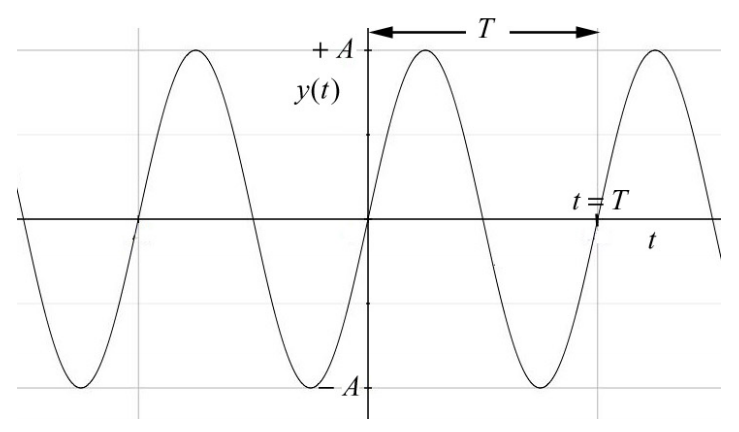
\includegraphics[scale=0.4]{graph.png}$$
	\caption{Sinusoidal function of time}
	\label{fig:Sinusoidal function of time}
\end{figure}

The sine function is periodic in time. This means that the value of the 
function at time $t$ will be exactly the same at a later time $t′ = t + T$ , 
where $T$ is the period. The \textbf{frequency}, $f$, is defined to be

\begin{sagesilent}
var('T')
z = 1/T
\end{sagesilent}

\begin{equation}
f = \sage{z}
\end{equation}

The SI unit of frequency is inverse seconds, hertz [Hz]. The angular frequency 
of oscillation is defined to be 

\begin{sagesilent}
var('omega,T,pi,f')
z=2*pi/T
z1=2*pi*f
\end{sagesilent}

\begin{equation}
\sage{omega} = \sage{z} = \sage{z1}
\end{equation}

and is measured in radians per second. We therefore have several different 
mathematical representations for sinusoidal motion

\begin{sagesilent}
var('A,pi,T,t,omega,f')
y = function('y',t)
z=A*sin(2*pi*t/T)
z1=A*sin(2*pi*f*t)
z2=A*sin(omega*t)
\end{sagesilent}

\begin{equation}
\sage{y} = \sage{z} = \sage{z1} = \sage{z2}
\end{equation}

% Creating next section
\section{Simple Harmonic Motion: Analytic approach}
Our first example of a system that demonstrates simple harmonic motion is a 
spring object system on a frictionless surface, shown in
Figure \ref{fig:Spring-object system}


\begin{figure}[h!]
$$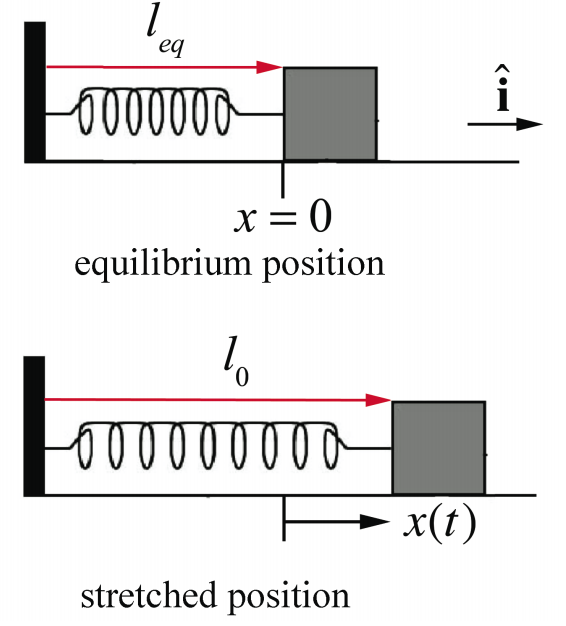
\includegraphics[scale=0.25]{diagram.png}$$
\caption{Spring-object system}
\label{fig:Spring-object system}
\end{figure}

The object is attached to one end of a spring. The other end of the spring is 
attached to a wall at the left in Figure \ref{fig:Spring-object system}.
Assume that the object undergoes 
one-dimensional motion. The spring has a spring constant $k$ and equilibrium 
length $l_{eq}$ . Choose the origin at the equilibrium position and choose the 
positive $x$ -direction to the right in the Figure \ref{fig:Spring-object system}.
In the figure, $x > 0$ 
corresponds to an extended spring, and $x < 0$ to a compressed spring. Define 
$x(t)$ to be the position of the object with respect to the equilibrium 
position. The force acting on the spring is a linear restoring force, $F_{x} = 
−k x$ (Figure ~\ref{Free-body force diagram for spring-object system}).
The initial conditions are as follows. The spring is 
initially stretched a distance $l_{0}$ and given some initial speed $v_{0}$ to 
the right away from the equilibrium position. The initial position of the 
stretched spring from the equilibrium position (our choice of origin) is $x_{0} 
= (l_{0}-l_{eq} ) > 0$ and its initial $x$ -component of the velocity is 
$v_{x,0} = v_{0} > 0$. 

\begin{figure}[h!]
$$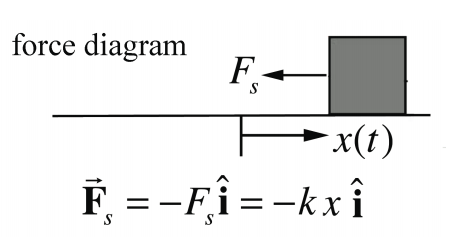
\includegraphics[scale=0.25]{diagram1.png}$$
\caption{Free-body force diagram for spring-object system}
\label{Free-body force diagram for spring-object system}
\end{figure}

Newton’s Second law in the $x$ -direction becomes

\begin{sagesilent}
var('k,t,m')
x = function('x',t)
z=-k*x
\end{sagesilent}

\begin{equation}
\sage{z} =  m\frac{\mathrm{d}^{2}x}{\mathrm{d}t^{2}}
\label{eq:1}
\end{equation}

This equation of motion, Eq.~\ref{eq:1}, is called the \textbf{simple harmonic 
oscillator equation} (SHO). Because the spring force depends on the distance 
$x$ , the acceleration is not constant. Eq.~\ref{eq:1} is a second order linear 
differential equation, in which the second derivative of the dependent variable 
is proportional to the negative of the dependent variable,

\begin{sagesilent}
z = -k*x/m
\end{sagesilent}

\begin{equation}
\frac{\mathrm{d}^{2}x}{\mathrm{d}t^{2}} = \sage{z}
\end{equation}

In this case, the constant of proportionality is $k/m$,

\begin{sagesilent}
# Declaring spring constant, mass, time as k, m, t respectively in SageMath
k=var('k')
m=var('m')
t=var('t')
x=function('x',t)

# Assuming spring constant and mass greater than zero
assume(k>0)
assume(m>0)

# Writing our differential equation in SageMath
de = diff(x,t,2)+(k*x)/m

# Soloving our differential equation in SageMath
z=desolve(de,dvar=x,ivar=t)
\end{sagesilent}

% Printing differential equation
\begin{equation}
  \frac{\mathrm{d}^{2}x}{\mathrm{d}t^{2}} +  \sage{k*x/m} = 0
\end{equation}

Since mass and spring constant cannot be negative and zero so, solving the 
above differential equation, we get,

\begin{equation}
x = \sage{z}
\label{eq:2}
\end{equation}

\begin{sagesilent}
# Declaring mass and spring constant equal to 1
m=1
k=1
de = diff(x,t,2)+k*x/m

# Soloving our differential equation by setting up the initial or boundary 
#conditions.
z2 = desolve(de,dvar=x,ivar=t,ics=[0,1,0])
# Plotting the graph of solution of our differential equation
pl1 = plot(z2,(t,0,10),color=('red'), figsize = 
(4,2.5),axes_labels=['$t$','$x$'], fontsize=7)

m=1
k=1
z3 = desolve(de,dvar=x,ivar=t,ics=[1,1,0])
print z3
pl2 = plot(z3,(t,0,10), color=('green'))

m=1
k=1
z4 = desolve(de,dvar=x,ivar=t, ics=[0,0,1])
pl3 = plot(z4,(t,0,10),color=('yellow'))

m=1
k=1
z5 = desolve(de,dvar=x,ivar=t, ics=[1,1,1])
pl4 = plot(z5,(t,0,10),color=('violet'))
\end{sagesilent}

For $m=1$ and $k=1$, then the graph is shown by Figure 
\ref{fig:Displacement Time graph1}.
\begin{figure}[h!]
% Ploting graph by using sage
$$\sageplot{pl1+pl2+pl3+pl4}$$
\caption{Displacement Time graph}
\label{fig:Displacement Time graph1}
\end{figure}
Here red, green, yellow and violet curves represents the initial or boundary 
conditions [0, 1, 0], [1, 1, 0], [0, 0, 1] and [1, 1, 1] respectively. Putting 
these initial conditions in Eq.~\ref{eq:2} one by one. Here $t$ corresponds to first 
term, $x$ corresponds to second term and $\frac{\mathrm{d}x}{\mathrm{d}t}$ 
corresponds to third term in the initial conditions.
